\begin{figure*}[t]
\providecommand{\width}{}
\renewcommand{\width}{0.15\textwidth}
\centering
\begin{subfigure}[t]{\width}
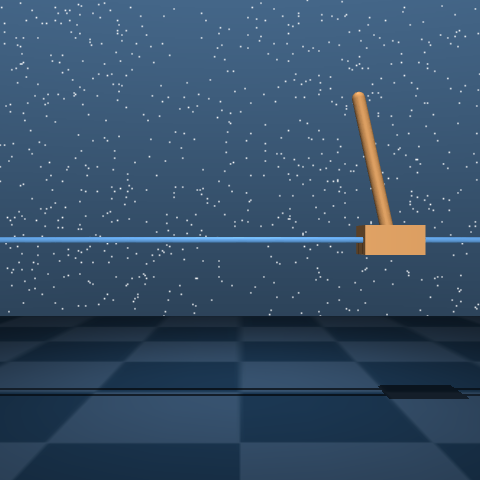
\includegraphics[width=\textwidth]{figures/domains/cartpole}
\caption{Cartpole}
\end{subfigure}\hfill%
\begin{subfigure}[t]{\width}
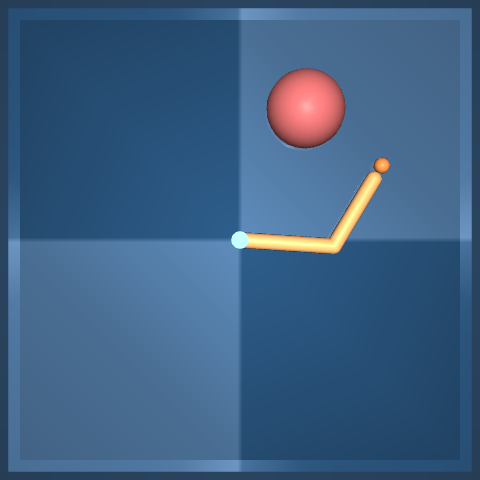
\includegraphics[width=\textwidth]{figures/domains/reacher}
\caption{Reacher}
\end{subfigure}\hfill%
\begin{subfigure}[t]{\width}
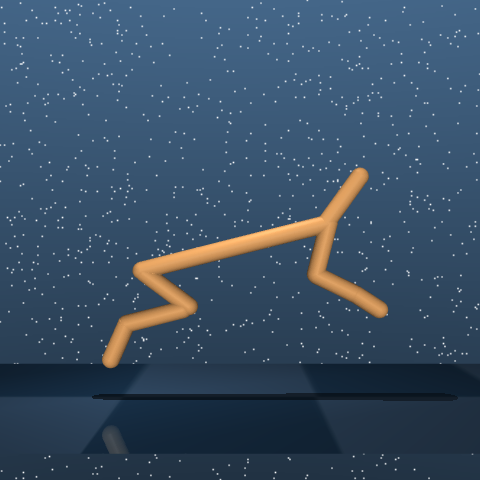
\includegraphics[width=\textwidth]{figures/domains/cheetah}
\caption{Cheetah}
\end{subfigure}\hfill%
\begin{subfigure}[t]{\width}
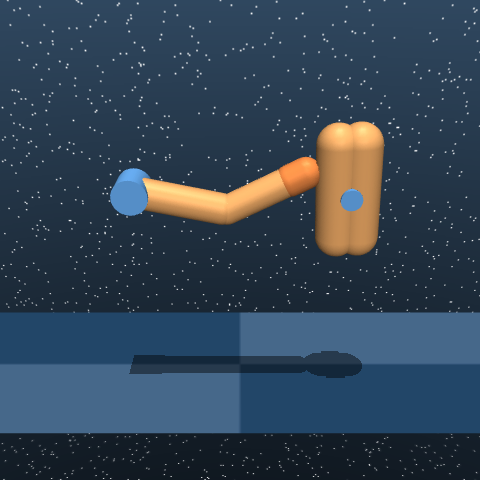
\includegraphics[width=\textwidth]{figures/domains/finger}
\caption{Finger}
\end{subfigure}\hfill%
\begin{subfigure}[t]{\width}
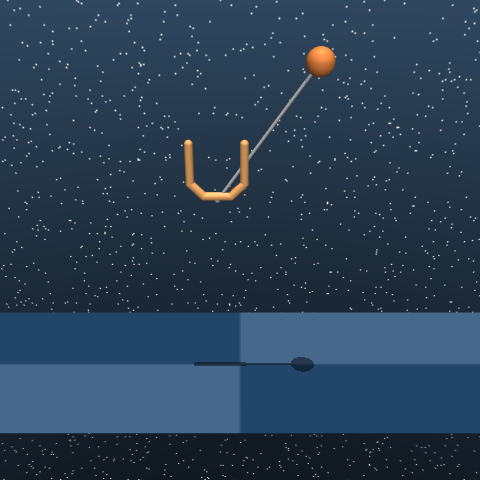
\includegraphics[width=\textwidth]{figures/domains/cup}
\caption{Cup}
\end{subfigure}\hfill%
\begin{subfigure}[t]{\width}
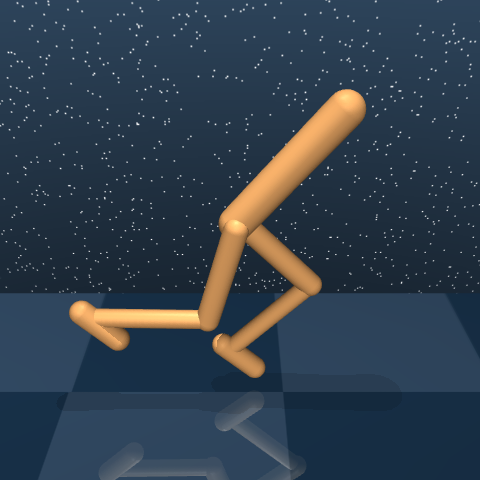
\includegraphics[width=\textwidth]{figures/domains/walker}
\caption{Walker}%
\end{subfigure}%
\caption{Image-based control domains used in our experiments. The images show agent observations before downscaling to $64\times 64\times 3$ pixels.
(a) The cartpole swingup task has a fixed camera so the cart can move out of sight.
(b) The reacher task has only a sparse reward.
(c) The cheetah running task includes both contacts and a larger number of joints.
(d) The finger spinning task includes contacts between the finger and the object.
(e) The cup task has a sparse reward that is only given once the ball is caught.
(f) The walker task requires balance and predicting difficult interactions with the ground when the robot is lying down.}
\label{fig:domains}
\end{figure*}
